\documentclass[letter,twoside,11pt]{report}

\usepackage[spanish,es-nodecimaldot]{babel}
\usepackage[utf8]{inputenc}

\usepackage{lmodern}
\usepackage[T1]{fontenc}
\usepackage{textcomp}

\usepackage{framed}
\usepackage[svgnames]{xcolor}
\colorlet{shadecolor}{Gainsboro!50}

\usepackage[labelfont=bf]{caption}
\usepackage{graphicx}
\usepackage{pstricks}

\usepackage{anysize}
\marginsize{3cm}{2cm}{2cm}{3cm}

\usepackage{siunitx}
\usepackage{amsmath}
\usepackage{array}
\usepackage{csquotes}
\usepackage{amsfonts}

\usepackage{fancyhdr}
\usepackage{lastpage}
\pagestyle{fancy}
\fancyhf{}
\fancyhead[LE,RO]{Laboratorio de Electrónica Analógica I}
\fancyfoot[CO,CE]{\thepage\ de \pageref{LastPage}}

\special{papersize=215.9mm,279.4mm}

\setcounter{tocdepth}{3}
\setcounter{secnumdepth}{3}

\usepackage[
    pdfauthor={Carlos Eduardo Caballero Burgoa},%
    pdftitle={Laboratorio de Electrónica Analógica I},%
    pdfsubject={Fuente de alimentación de corriente directa},%
    colorlinks,%
    citecolor=black,%
    filecolor=black,%
    linkcolor=black,%
    urlcolor=black,
    breaklinks]{hyperref}
\usepackage{breakurl}

\newcommand{\blankpage}{
\newpage
\thispagestyle{empty}
\mbox{}
\newpage
}

\renewcommand{\arraystretch}{1.2}
\renewcommand{\thesection}{\arabic{section}}

\begin{document}

\begin{titlepage}
    \begin{center}
        {\Large UNIVERSIDAD MAYOR DE SAN SIMÓN}\\
        \vspace*{0.15cm}
        {\large FACULTAD DE CIENCIAS Y TECNOLOGÍA}\\
        \vspace*{0.10cm}
        DEPARTAMENTO DE ELÉCTRICA-ELECTRÓNICA\\
        \vspace*{3.0cm}
        {\Large \textbf{LABORATORIO DE ELECTRÓNICA ANALÓGICA I}}\\
        \vspace*{0.3cm}
        {\Large \textbf{INFORME No. 2}}\\
        \vspace*{3.5cm}
        {\Large \textbf{FUENTE DE ALIMENTACIÓN DE \\
        CORRIENTE DIRECTA}}\\
    \end{center}

    \vspace*{5.8cm}
    \leftskip=7.95cm
    \noindent
    \textbf{Estudiante:}\\
    Caballero Burgoa, Carlos Eduardo.\\
    \newline
    \textbf{Carrera:}\\
    Ing. Electromecánica.\\
    \newline
    \textbf{Docente:}\\
    Ing. Alberto Arispe Santander.\\
    \newline
    \textbf{Grupo:} 1B.\\
    \textbf{Fecha de entrega:} 5 de Noviembre del 2024.\\
\end{titlepage}
\addtocounter{page}{-1}

\blankpage
\addtocounter{page}{-1}

\tableofcontents
\newpage

\section{Introducción}
Todos los dispositivos electrónicos activos requieren una fuente de corriente
directa (CD) constante que provenga de una batería o una fuente de
alimentación. La \textbf{fuente de alimentación de CD} convierte el voltaje de
corriente alterna (CA) estándar de $220[\text{V}]$ a $50[\text{Hz}]$ disponible
en las tomas de corriente de pared en un voltaje de CD constante.

En la \textbf{figura~\ref{diagrama}} se muestra un diagrama de bloques básico de
una fuente de alimentación completa.

\begin{figure}[!h]
\centering
\includegraphics[scale=1.50]{diagramas/00.diagrama.eps}
\caption{Fuente de alimentación completa.}
\label{diagrama}
\end{figure}

En general, el voltaje de linea de entrada de CA se reduce a un voltaje de CA
más bajo con un \textbf{transformador}. Este cambia voltajes de CA con base en
la relación de vueltas entre el primario y el secundario. Si éste tiene más
vueltas que el primario, el voltaje de salida a través del secundario será más
alto y la corriente será más pequeña. Si el secundario tiene menos vueltas que
el primario, el voltaje de salida a través del secundario será más bajo y la
corriente será más alta.

El \textbf{rectificador} puede ser de media onda o de onda completa, este
convierte el voltaje de entrada de CA en un voltaje de CD pulsante.

El \textbf{filtro} elimina los rizos de voltaje en el rectificador y produce un
voltaje de CD relativamente uniforme.

El \textbf{regulador} es un circuito que mantiene un voltaje de CD constante
frente a las variaciones de voltaje de linea de entrada o de la carga. Los
reguladores varían desde un dispositivo de un solo semiconductor hasta circuitos
integrados mas complejos.

La \textbf{carga} es un circuito o dispositivo conectado a la salida de la
fuente de alimentación y opera con el voltaje y la corriente de la fuente de
alimentación \cite{Floyd}.


\section{Objetivos}
\begin{itemize}
    \item Verificar el comportamiento de los transformadores con derivación
        central.
    \item Verificar el comportamiento de los rectificadores de media onda y onda
        completa.
    \item Verificar el comportamiento de los rectificadores con filtro.
    \item Verificar el comportamiento de los reguladores de voltaje.
\end{itemize}


\section{Transformador}
A menudo se utiliza un transformador para acoplar el voltaje de entrada de ca
proveniente de la fuente al rectificador. El acoplamiento por transformador
ofrece dos ventajas:

\begin{itemize}
    \item Permite que la fuente de voltaje se reduzca como sea necesario.
    \item La fuente de ca se aísla eléctricamente del rectificador, con lo que
        se evita el peligro de choques eléctricos en el circuito del
        secundario \cite{Floyd}.
\end{itemize}

Se utilizará un transformador de $220[\text{V}]$ a $12[\text{V}]$ con derivación
central de $1[\text{A}]$, con los voltajes descritos en la
\textbf{figura~\ref{circuito01}}.

\begin{figure}[!h]
\centering
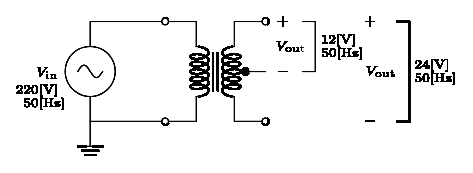
\includegraphics[scale=1]{diagramas/01.transformador.eps}
\caption{Voltajes de entrada y salida del transformador.}
\label{circuito01}
\end{figure}

\subsection{Simulación}
Se utilizó el software \emph{Quite Universal Circuit Simulator.} versión 23.3.1
para la simulación del transformador, este puede verse en la
\textbf{figura~\ref{simulacion01}}.

\begin{figure}[!h]
\centering
\includegraphics[scale=0.75]{simulacion/01.transformador.eps}
\caption{Simulación del transformador de $220[\text{V}]$ a $12[\text{V}]$.}
\label{simulacion01}
\end{figure}

\subsection{Laboratorio}
Para los experimentos se utilizó el transformador mostrado en la
\textbf{figura~\ref{laboratorio01}}.

\begin{figure}[!h]
\centering
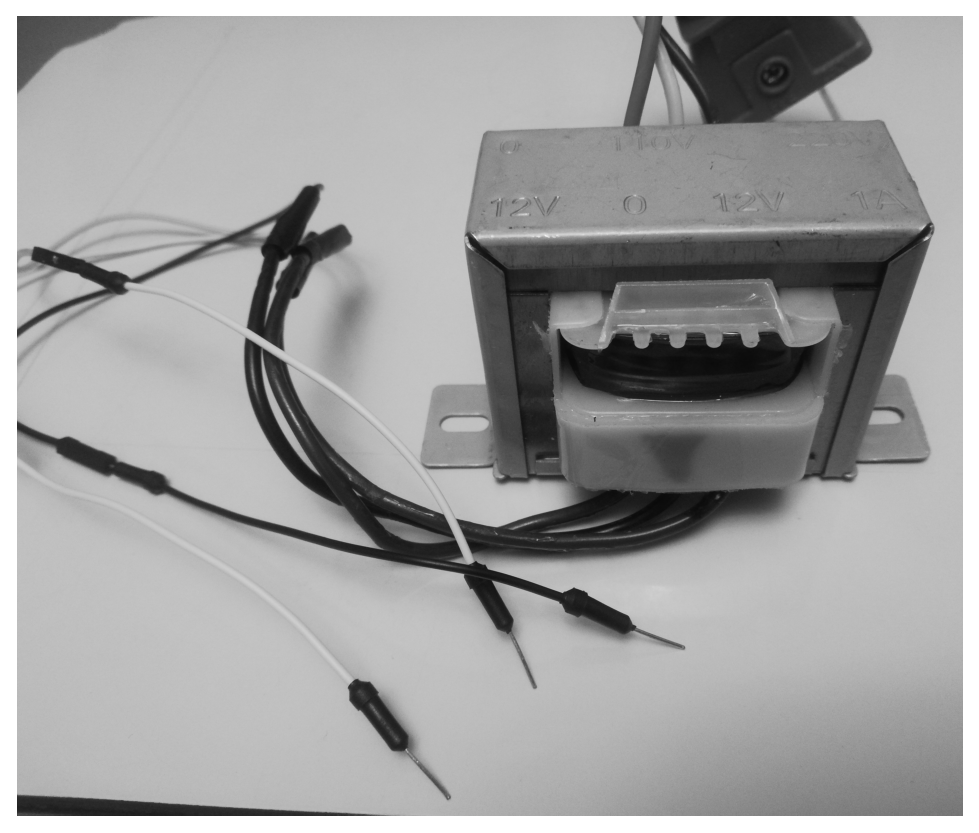
\includegraphics[scale=0.28]{fotos/01.transformador1.eps}
\caption{Transformador con derivación central.}
\label{laboratorio01}
\end{figure}

El transformador puede usarse para disponer de una salida de $12[\text{V}]$ o
una de $24[\text{V}]$, segun se utilizen dos de sus tres terminales, como puede
verse en la \textbf{figura~\ref{laboratorio02}} y la
\textbf{figura~\ref{laboratorio03}} respectivamente.

\begin{figure}[!h]
\centering
\includegraphics[scale=0.28]{fotos/01.transformador2.eps}
\caption{Señal de salida del transformador a $12[\text{V}]$.}
\label{laboratorio02}
\end{figure}

\begin{figure}[!h]
\centering
\includegraphics[scale=0.28]{fotos/01.transformador3.eps}
\caption{Señal de salida del transformador a $24[\text{V}]$.}
\label{laboratorio03}
\end{figure}


\section{Rectificador}
La rectificación es el proceso de convertir una forma de onda de corriente
alterna en una forma de onda de corriente continua (en este caso, variable) que
tiene una sola polaridad.

\subsection{Media onda}
Considerando el circuito de la \textbf{figura~\ref{circuito02}}, se aprecia un
bucle en serie que consiste en una fuente de onda sinusoidal conectada a un
transformador; desde el transformador se conecta un diodo \textbf{1N4007} y una
resistencia de $10[\text{k}\Omega]$ que cumple la función de carga.

\begin{figure}[!h]
\centering
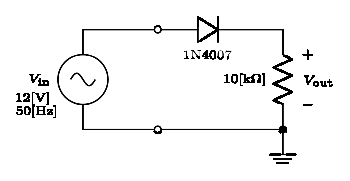
\includegraphics[scale=1.1]{diagramas/02.media_onda1.eps}
\caption{Rectificador de media onda.}
\label{circuito02}
\end{figure}

Para los valores positivos del voltaje de entrada, el diodo estará polarizado
directamente, por tanto la señal de entrada caerá a través de la resistencia de
carga; mientras que con los valores negativos del voltaje de entrada, hará que
el diodo este polarizado inversamente y por tanto no circulará corriente a
través de la carga.

\subsubsection{Simulación}
Se utilizó el software \emph{Quite Universal Circuit Simulator.} versión 23.3.1
para la simulación del rectificador de media onda, este puede verse en la
\textbf{figura~\ref{simulacion02}}.

\begin{figure}[!h]
\centering
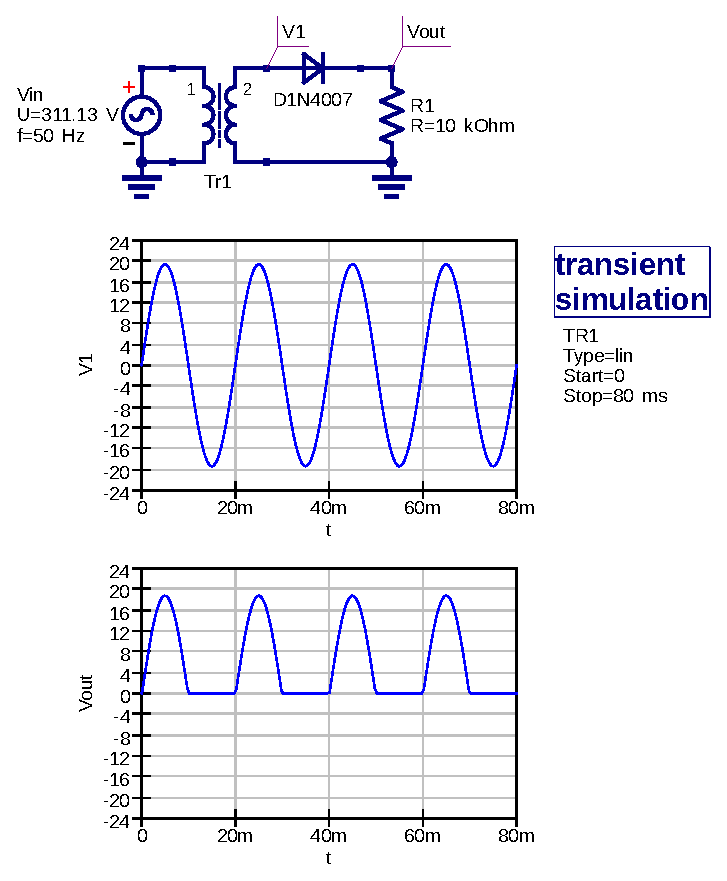
\includegraphics[scale=0.75]{simulacion/02.media_onda1.eps}
\caption{Simulación del rectificador de media onda.}
\label{simulacion02}
\end{figure}

\subsubsection{Laboratorio}
Se presenta el rectificador de media onda armado en laboratorio y su medición
de voltaje de salida en la carga, en la \textbf{figura~\ref{laboratorio04}}.

\begin{figure}[!h]
\centering
\includegraphics[scale=0.34]{fotos/02.media_onda1.eps}
\caption{Rectificador de media onda.}
\label{laboratorio04}
\end{figure}


\subsection{Onda completa con derivación central}
Este rectificador utiliza dos diodos \textbf{1N4007} conectados a un
transformador con derivación central y una resistencia de $10[\text{k}\Omega]$
que cumple la función de carga, como se muestra en la
\textbf{figura~\ref{circuito03}}, los voltajes entre las terminales del
transformador son iguales en magnitud, pero con diferentes fases.

\begin{figure}[!h]
\centering
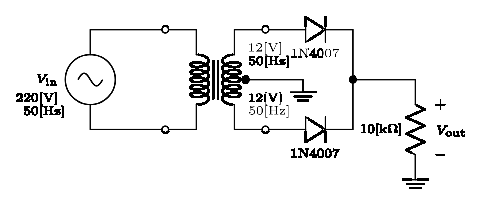
\includegraphics[scale=1.1]{diagramas/03.derivacion_central1.eps}
\caption{Rectificador de onda completa con transformador de derivación central.}
\label{circuito03}
\end{figure}

La polarización directa e inversa son alternadas en cada diodo del circuito por
lo que se obtienen solo los valores positivos de cada extremo del transformador.

\subsubsection{Simulación}
Se utilizó el software \emph{Quite Universal Circuit Simulator.} versión 23.3.1
para la simulación del rectificador de onda completa, este puede verse en la
\textbf{figura~\ref{simulacion03}}.

\begin{figure}[!h]
\centering
\includegraphics[scale=0.75]{simulacion/03.derivacion_central1.eps}
\caption{Simulación del rectificador de onda completa con derivación central.}
\label{simulacion03}
\end{figure}

\subsubsection{Laboratorio}
Se presenta el rectificador de onda completa con el transformador de derivación
central armado en laboratorio y su medición de voltaje de salida en la carga, en
la \textbf{figura~\ref{laboratorio05}}.

\begin{figure}[!h]
\centering
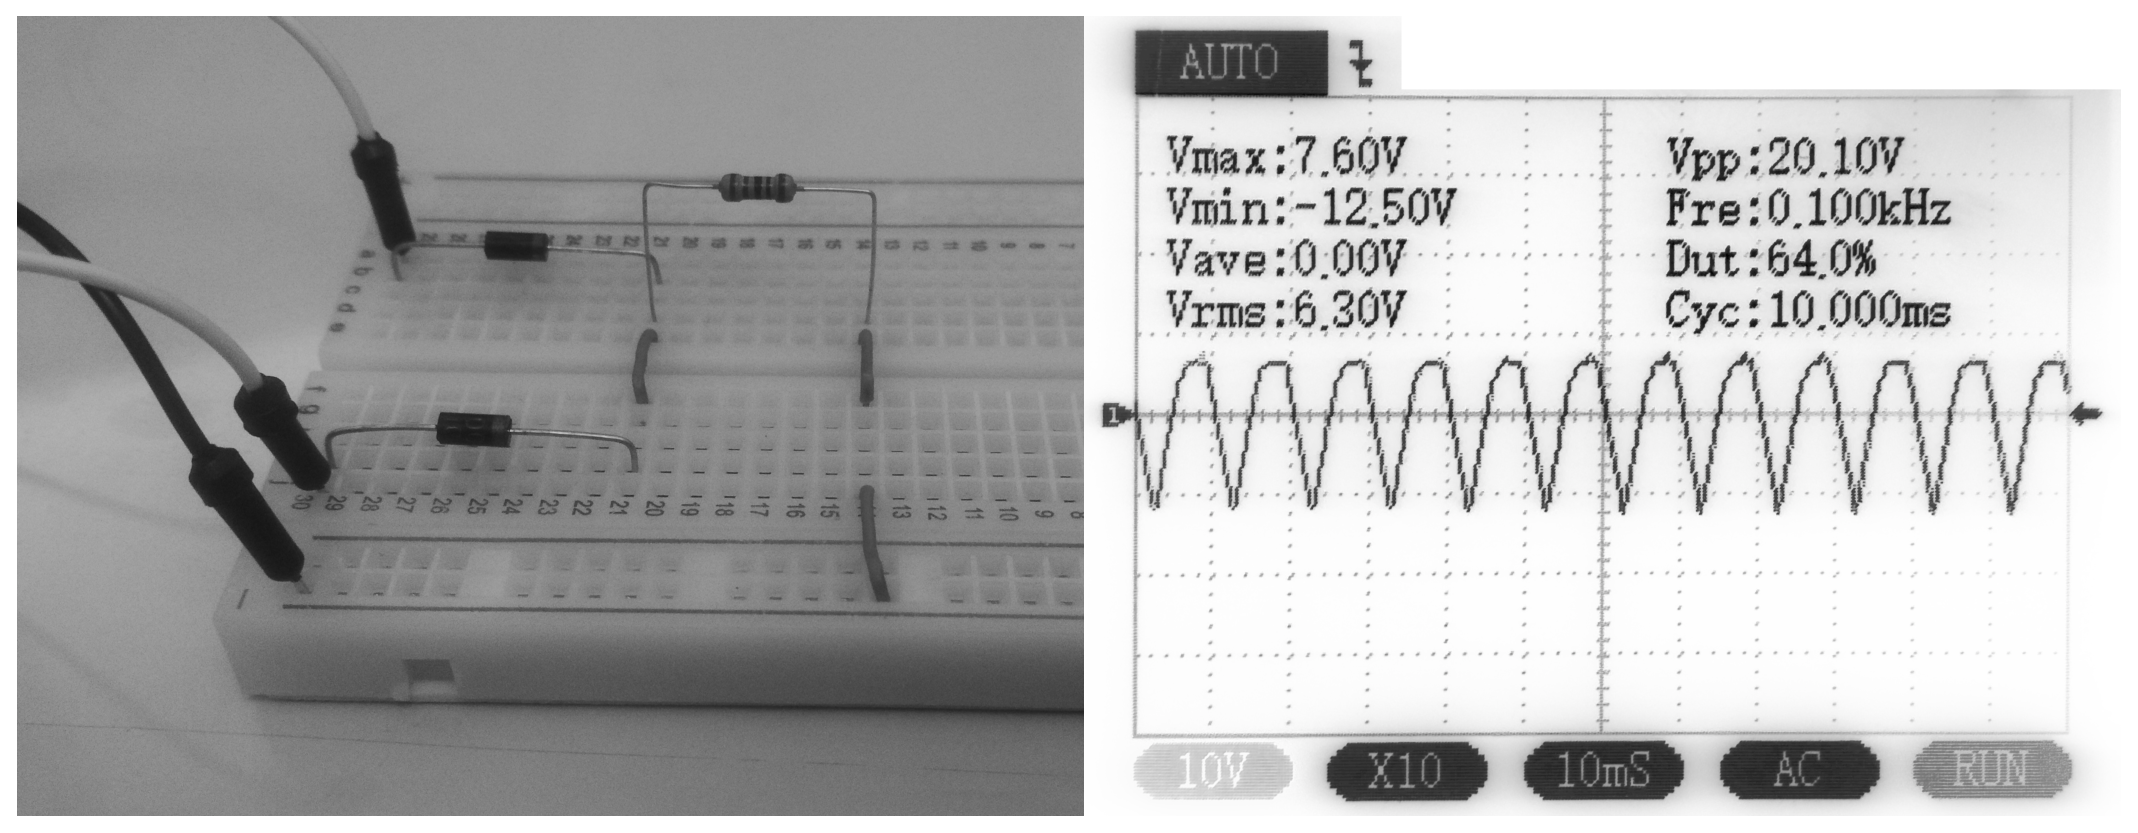
\includegraphics[scale=0.34]{fotos/03.derivacion_central1.eps}
\caption{Rectificador de onda completa con derivación central.}
\label{laboratorio05}
\end{figure}


\subsection{Onda completa de puente}
Este rectificador utiliza cuatro diodos \textbf{1N4007} conectados como un
puente y conectados a una resistencia de $10[\text{k}\Omega]$, como se muestra
en la \textbf{figura~\ref{circuito04}}.

\begin{figure}[!h]
\centering
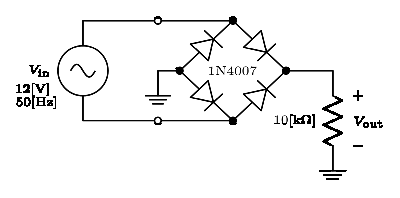
\includegraphics[scale=1.1]{diagramas/04.onda_completa1.eps}
\caption{Rectificador de onda completa con puente.}
\label{circuito04}
\end{figure}

Los valores positivos del voltaje de entrada polariza directamente a dos diodos
y polariza inversamente a los dos diodos restantes, mientras que los valores
negativos del voltaje hace el camino contrario por los diodos del circuito, lo
que genera la señal de onda completa con el doble de la frecuencia del voltaje
de entrada.

\subsubsection{Simulación}
Se utilizó el software \emph{Quite Universal Circuit Simulator.} versión 23.3.1
para la simulación del rectificador de onda completa, este puede verse en la
\textbf{figura~\ref{simulacion04}}.

\begin{figure}[!h]
\centering
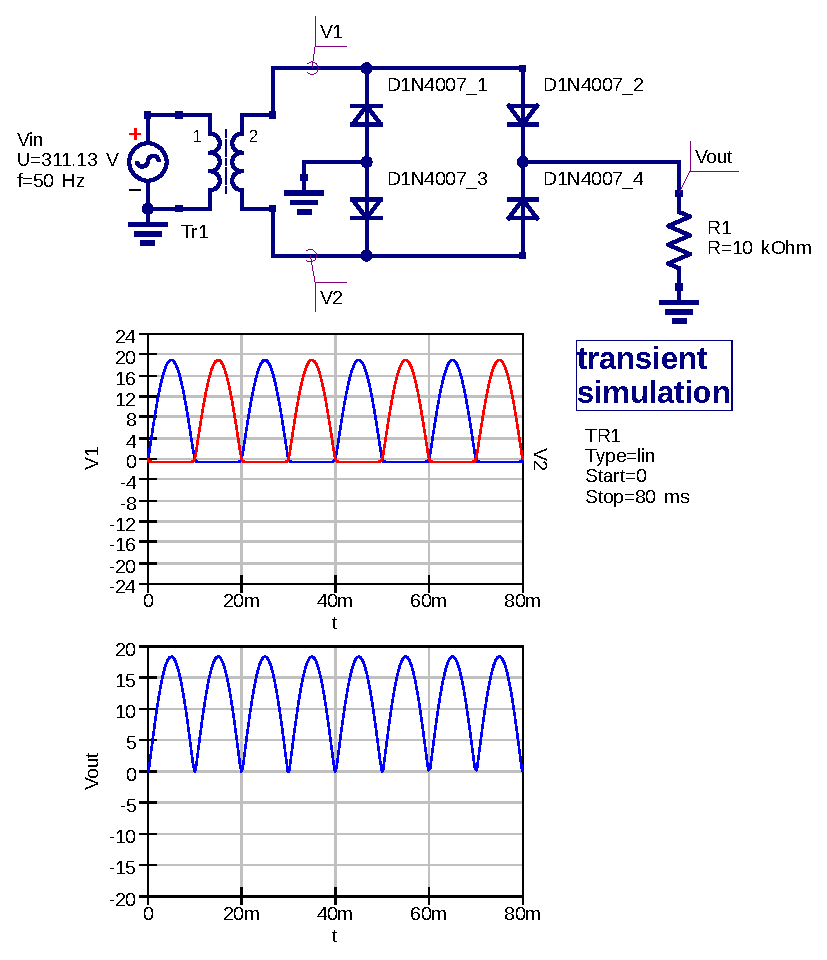
\includegraphics[scale=0.75]{simulacion/04.onda_completa1.eps}
\caption{Simulación del rectificador de onda completa con puente.}
\label{simulacion04}
\end{figure}

\subsubsection{Laboratorio}
Se presenta el rectificador de onda completa con puente armado en laboratorio y
su medición de voltaje de salida en la carga, en la
\textbf{figura~\ref{laboratorio06}}.

\begin{figure}[!h]
\centering
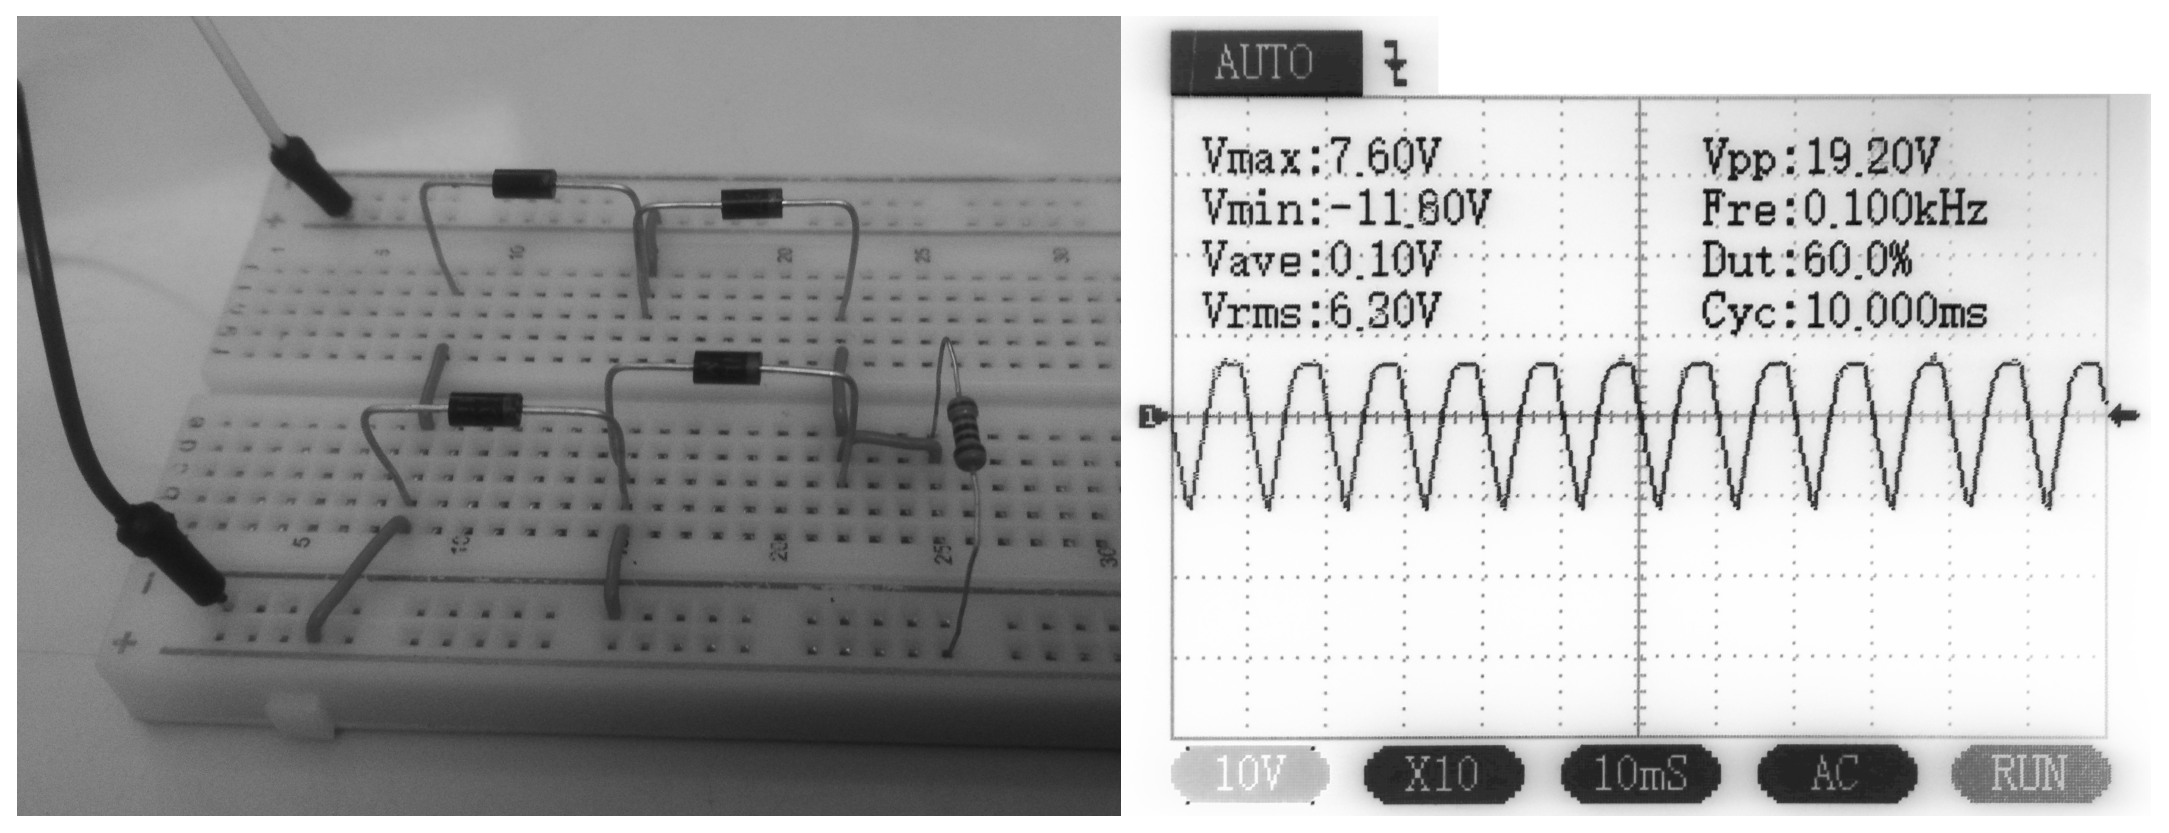
\includegraphics[scale=0.34]{fotos/04.onda_completa1.eps}
\caption{Rectificador de onda completa con puente.}
\label{laboratorio06}
\end{figure}


\section{Filtro}
Una vez rectificada la señal el siguiente paso es suavizar y nivelar la
corriente directa pulsante. El método más sencillo para lograr esto es agregar
un condensador en paralelo a la carga. El condensador se cargará durante la fase
de conducción, almacenando así energía. Cuando el diodo se apaga, el condensador
comenzará a descargarse, transfiriendo así su energía almacenada a la carga.

\subsection{Media onda}
El circuito con filtro de $470[\mu\text{F}]$ pueden verse en la
\textbf{figura~\ref{circuito05}} para el rectificador de media onda.

\begin{figure}[!h]
\centering
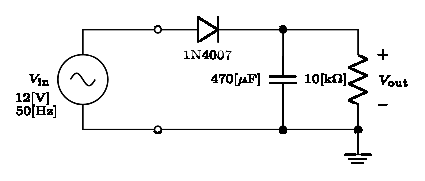
\includegraphics[scale=1.1]{diagramas/05.media_onda2.eps}
\caption{Rectificador de media onda con filtro.}
\label{circuito05}
\end{figure}

\subsubsection{Simulación}
Se utilizó el software \emph{Quite Universal Circuit Simulator.} versión 23.3.1
para la simulación del rectificador de media onda con filtro, este puede verse
en la \textbf{figura~\ref{simulacion05}}.

\begin{figure}[!h]
\centering
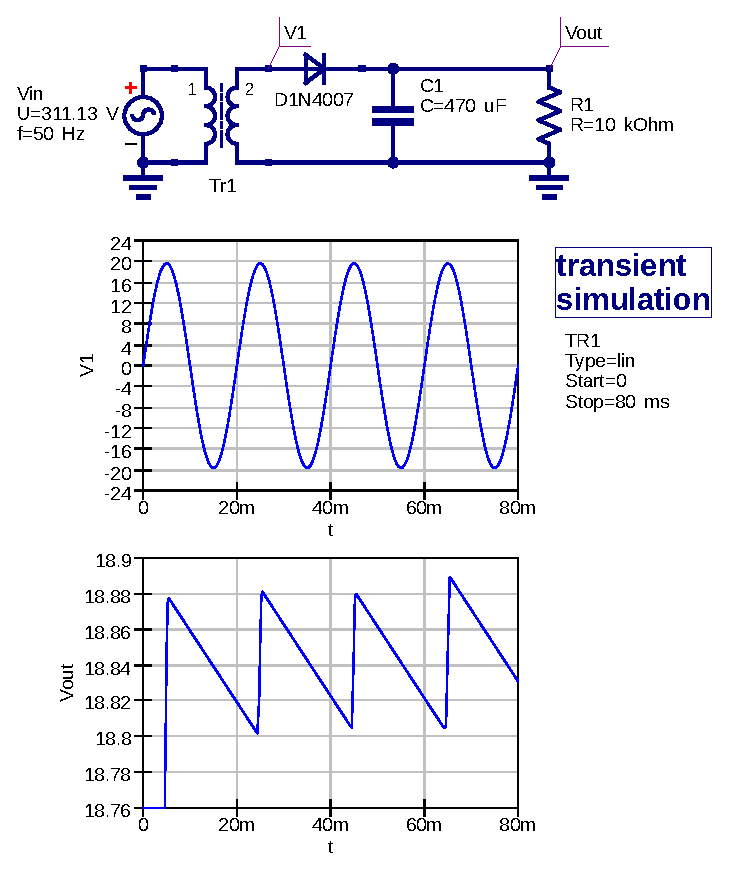
\includegraphics[scale=0.75]{simulacion/05.media_onda2.eps}
\caption{Simulación del rectificador de media onda con filtro.}
\label{simulacion05}
\end{figure}

\subsubsection{Laboratorio}
Se presenta el rectificador de media onda con filtro armado en laboratorio y su
medición de voltaje de salida en la carga, en la
\textbf{figura~\ref{laboratorio07}}.

\begin{figure}[!h]
\centering
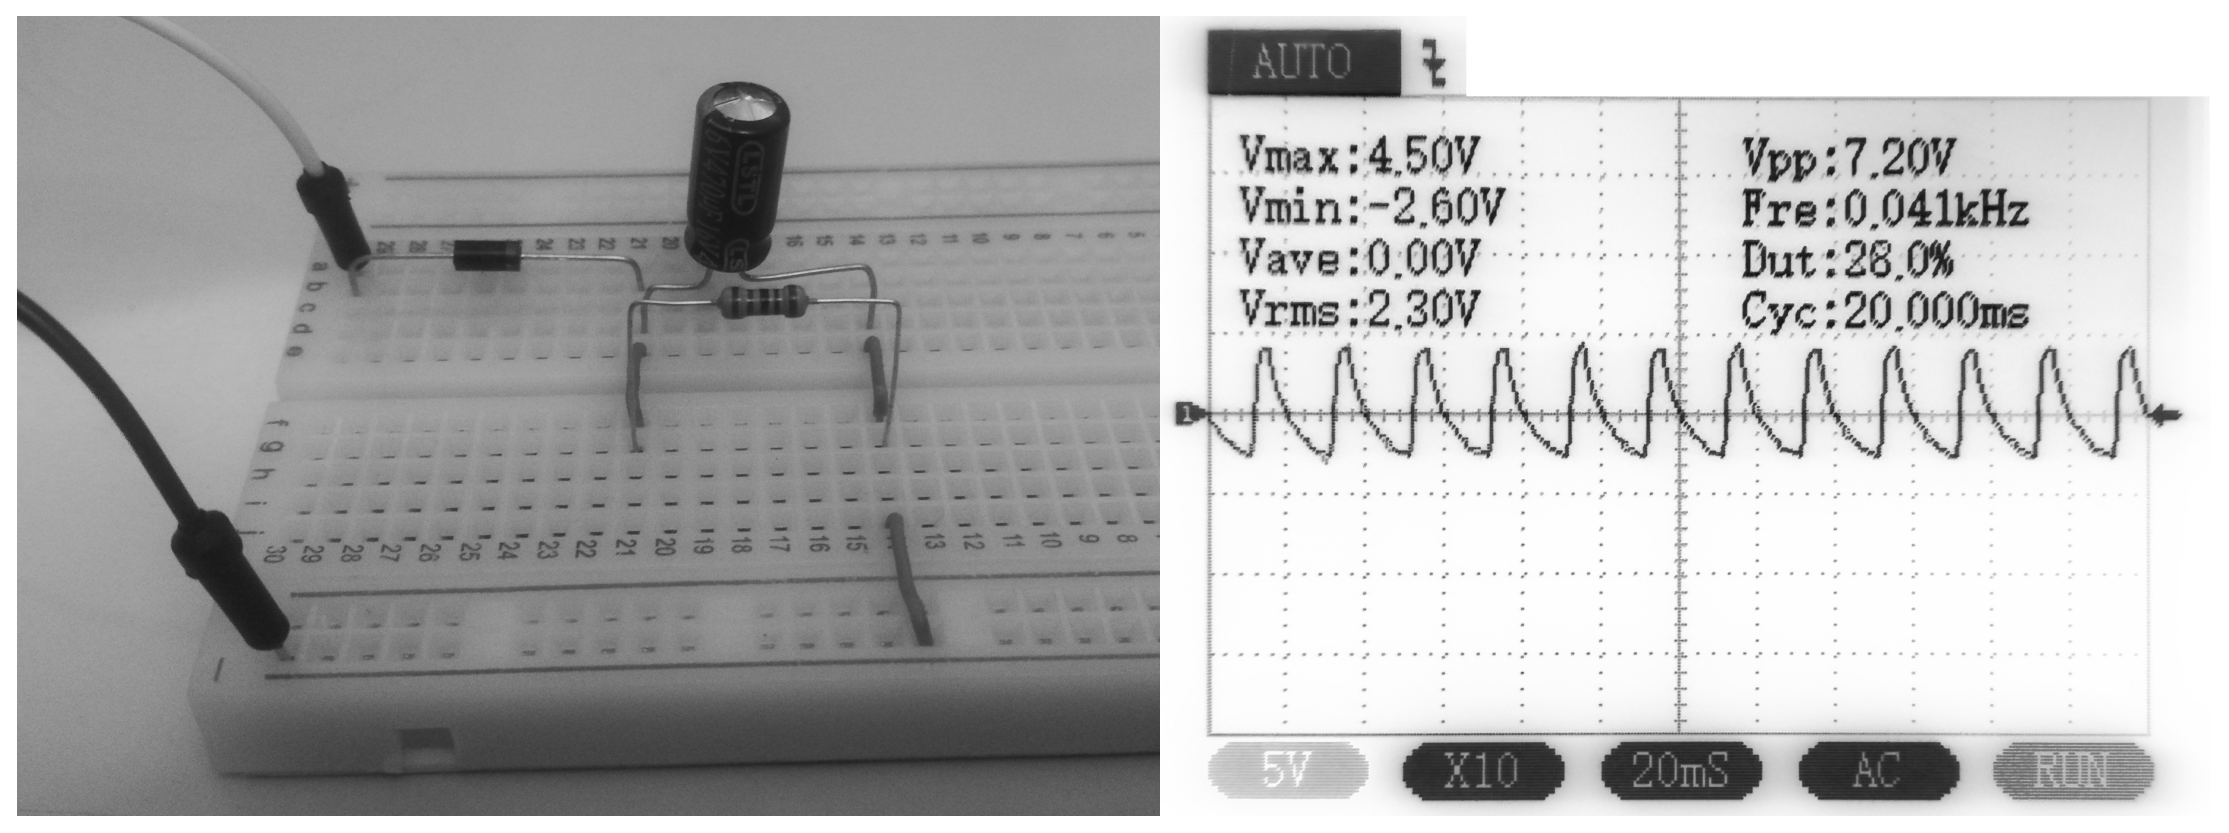
\includegraphics[scale=0.34]{fotos/05.media_onda2.eps}
\caption{Rectificador de media onda con filtro.}
\label{laboratorio07}
\end{figure}


\subsection{Onda completa con derivación central}
El circuito con filtro de $470[\mu\text{F}]$ pueden verse en la
\textbf{figura~\ref{circuito06}} para el rectificador de onda completa con
derivación central.

\begin{figure}[!h]
\centering
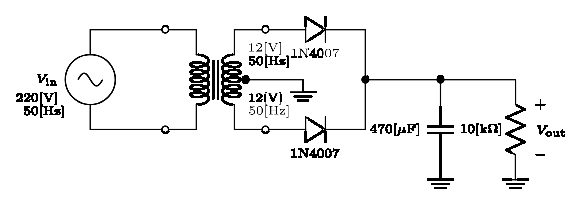
\includegraphics[scale=1.1]{diagramas/06.derivacion_central2.eps}
\caption{Rectificador de onda completa con transformador de \\
derivación central y filtro.}
\label{circuito06}
\end{figure}

\subsubsection{Simulación}
Se utilizó el software \emph{Quite Universal Circuit Simulator.} versión 23.3.1
para la simulación del rectificador de onda completa con transformador de
derivación central con filtro, este puede verse en la
\textbf{figura~\ref{simulacion06}}.

\begin{figure}[!h]
\centering
\includegraphics[scale=0.75]{simulacion/06.derivacion_central2.eps}
\caption{Simulación del rectificador de onda completa con \\
derivación central y filtro.}
\label{simulacion06}
\end{figure}

\subsubsection{Laboratorio}
Se presenta el rectificador de onda completa con el transformador de derivación
central y filtro armado en laboratorio y su medición de voltaje de salida en la
carga, en la \textbf{figura~\ref{laboratorio08}}.

\begin{figure}[!h]
\centering
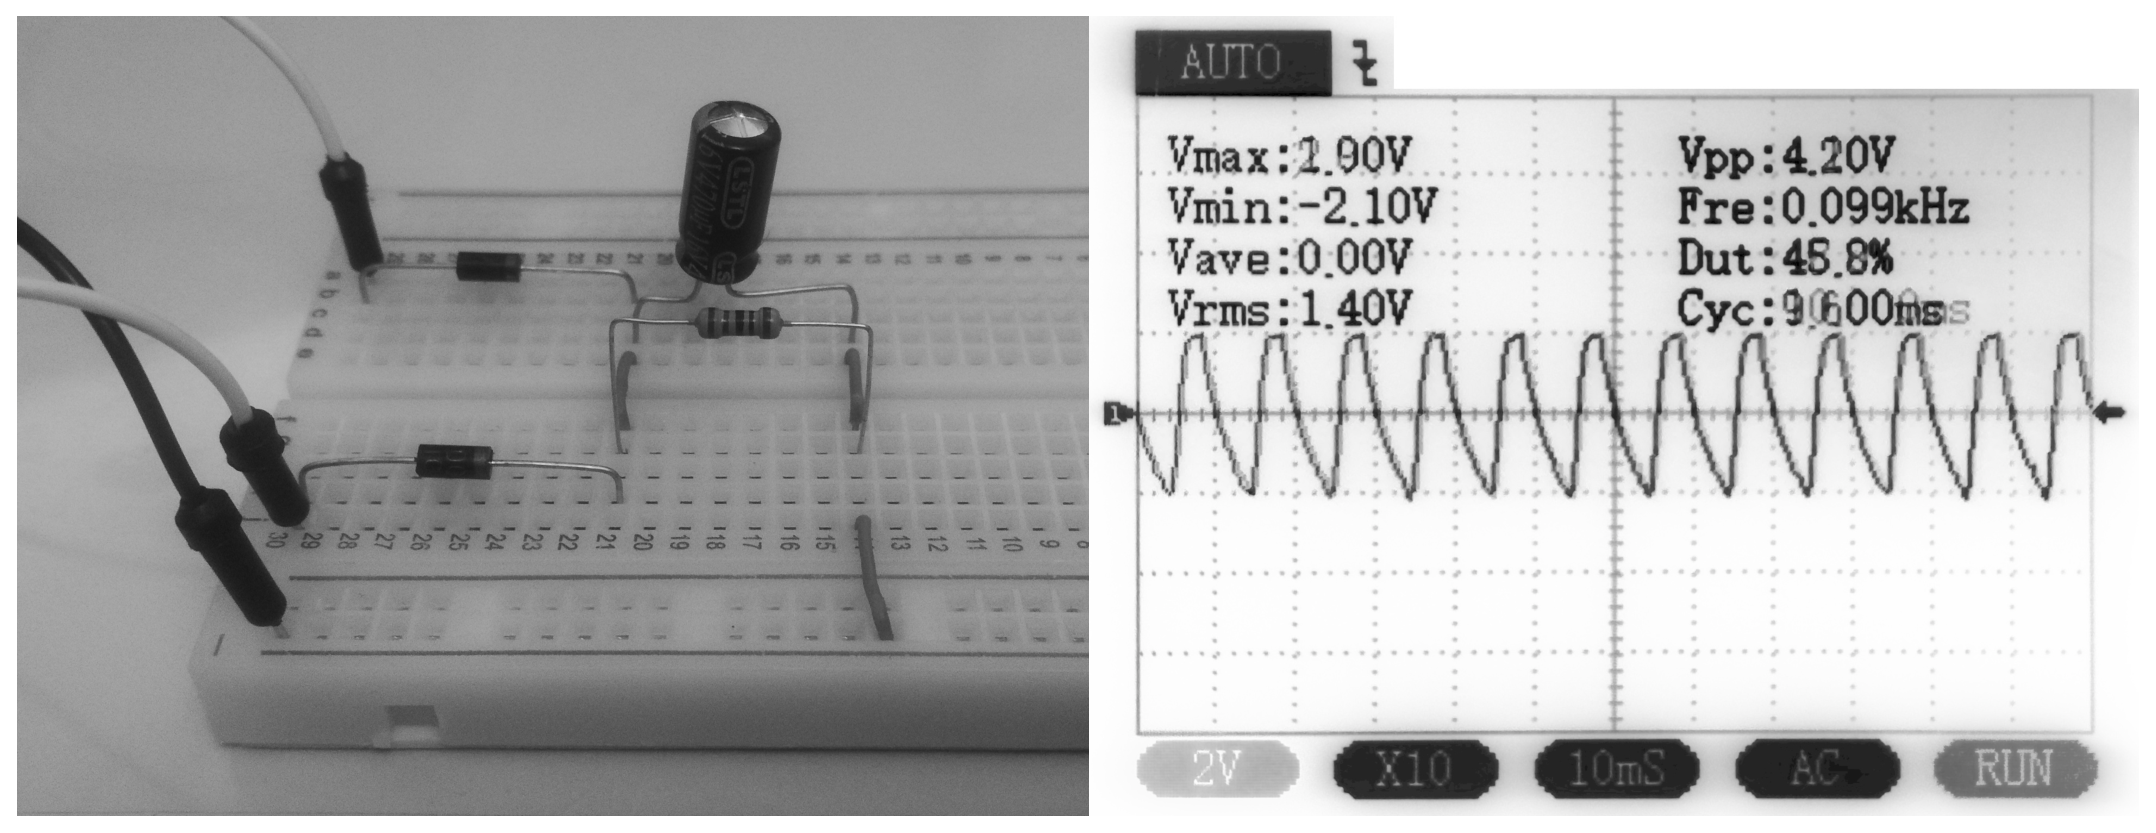
\includegraphics[scale=0.34]{fotos/06.derivacion_central2.eps}
\caption{Rectificador de onda completa con derivación central y filtro.}
\label{laboratorio08}
\end{figure}


\subsection{Onda completa de puente}
El circuito con filtro de $470[\mu\text{F}]$ pueden verse en la
\textbf{figura~\ref{circuito07}} para el rectificador de onda completa de
puente.

\begin{figure}[!h]
\centering
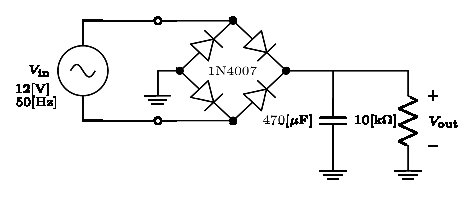
\includegraphics[scale=1.1]{diagramas/07.onda_completa2.eps}
\caption{Rectificador de onda completa con puente y filtro.}
\label{circuito07}
\end{figure}

\subsubsection{Simulación}
Se utilizó el software \emph{Quite Universal Circuit Simulator.} versión 23.3.1
para la simulación del rectificador de onda completa con filtro, este puede
verse en la \textbf{figura~\ref{simulacion07}}.

\begin{figure}[!h]
\centering
\includegraphics[scale=0.75]{simulacion/07.onda_completa2.eps}
\caption{Simulación del rectificador de onda completa con puente y filtro.}
\label{simulacion07}
\end{figure}

\subsubsection{Laboratorio}
Se presenta el rectificador de onda completa con puente y filtro armado en
laboratorio y su medición de voltaje de salida en la carga, en la
\textbf{figura~\ref{laboratorio09}}.

\begin{figure}[!h]
\centering
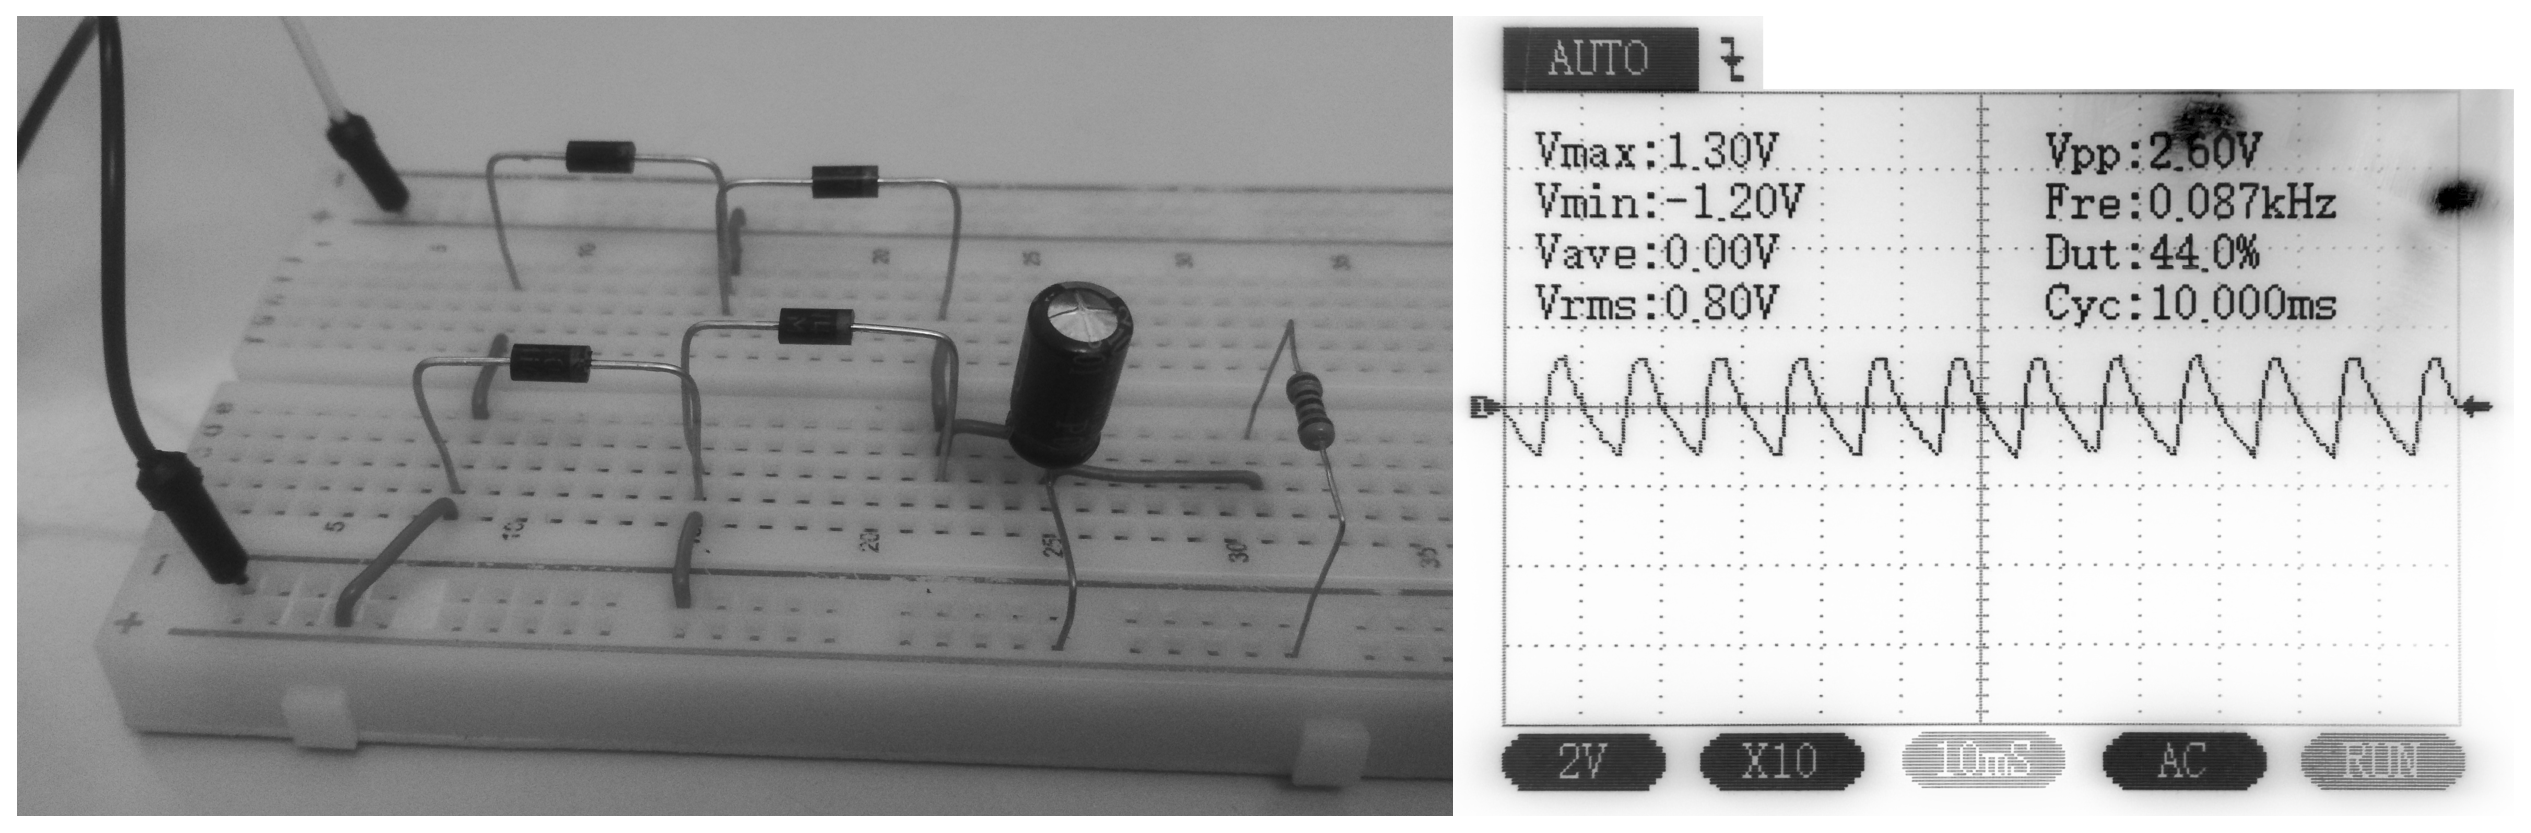
\includegraphics[scale=0.34]{fotos/07.onda_completa2.eps}
\caption{Rectificador de onda completa con puente y filtro.}
\label{laboratorio09}
\end{figure}


\section{Regulador de voltaje}
Mientras los filtros pueden reducir la fluctuación de las fuentes de
alimentación, el método más efectivo es una combinación de un filtro de entrada
con capacitor utilizado con un regulador de voltaje. Se conecta un regulador de
voltaje a la salida de un rectificador filtrado y mantiene un voltaje de salida
constante. El filtro de entrada con capacitor reduce el rizo de entrada al
regulador a un nivel aceptable. La combinación de un capacitor grande y un
regulador de voltaje ayudan a producir una excelente fuente de alimentación.

\subsection{Diodo \emph{Zener}}
Cuando se polariza hacia atrás con un potencial suficientemente grande, el
comportamiento normal del diodo inverso (de un interruptor abierto) cambia
abruptamente para mantener un voltaje fijo; \textbf{el potencial \emph{Zener}}.
La corriente a través del diodo comienza a aumentar drásticamente una vez que se
alcanza este potencial. Si se coloca un diodo \emph{Zener} a través de la salida
del rectificador filtrado, el \emph{Zener} intentará limitar el voltaje
de salida al potencial \emph{Zener}.

Para evitar el consumo excesivo y posiblemente destructivo de corriente por el
diodo \emph{Zener}, la diferencia de voltaje entre el voltaje del condensador y
el potencial \emph{Zener} se reduce a través de una resistencia limitadora de
corriente en serie. Esta resistencia limitadora establecerá la cantidad máxima
de corriente de salida. Esta corriente se divide entonces entre el diodo
\emph{Zener} y la carga.

Bajo condiciones de carga ligera, la mayor parte de esta corriente fluirá a
través del diodo \emph{Zener}. Bajo condiciones de carga pesada, la mayor parte
de la corriente será extraída por la carga con poco flujo a través del diodo
\emph{Zener}. Si la demanda de corriente de carga es demasiado pesada, no hay
corriente disponible para el diodo \emph{Zener} y deja de conducir. La
regulación se pierde y la resistencia limitadora forma un divisor de voltaje con
la carga \cite{Fiore}.

\subsubsection{Calculo de la resistencia limitadora}
Considerando el voltaje de entrada:
\begin{equation*}
    \begin{split}
        V_i &= 18\,\sen(100\pi\,t)[\text{V}]\\
    \end{split}
\end{equation*}

Se utilizará un diodo \emph{Zener} \textbf{1N4742A} con los siguientes
parámetros:
\begin{equation*}
    \begin{split}
        V_z &= 12[\text{V}]\\
        P_z &= 0.5[\text{W}]\\
    \end{split}
\end{equation*}

Se halla el intervalo aceptable de corriente:
\begin{equation*}
    \begin{split}
        I_{\text{max}} &= \frac{P_z}{V_z}\\
                       &= \frac{0.5}{12}\\
                       &= 41.67[\text{mA}]\\
        I_{\text{min}} &= 0.1\,I_{\text{max}}\\
                       &= 0.1\,41.67[\text{mA}]\\
                       &= 4.167[\text{mA}]\\
    \end{split}
\end{equation*}

Por tanto, los intervalos aceptables para la resistencia limitadora son:
\begin{equation*}
    \begin{split}
        R_{\text{max}} &= \frac{V_p - V_z}{I_{\text{max}}}\\
                       &= \frac{18 - 12}{0.041.67}\\
                       &= 144[\Omega]\\
    \end{split}
\end{equation*}
\begin{equation*}
    \begin{split}
        R_{\text{min}} &= \frac{V_p - V_z}{I_{\text{min}}}\\
                       &= \frac{18 - 12}{0.0041.67}\\
                       &= 1440[\Omega]\\
    \end{split}
\end{equation*}

El valor normalizado para la resistencia limitadora utilizado es
$1[\text{k}\Omega]$.

El circuito con filtro y con diodo \emph{Zener} puede verse en la
\textbf{figura~\ref{circuito08}}.

\begin{figure}[!h]
\centering
\includegraphics[scale=1.1]{diagramas/08.zener1.eps}
\caption{Regulación de voltaje con diodo \emph{Zener}.}
\label{circuito08}
\end{figure}

\subsubsection{Simulación}
Se utilizó el software \emph{Quite Universal Circuit Simulator.} versión 23.3.1
para la simulación de la regulación de voltaje con el diodo \emph{Zener}, este
puede verse en la \textbf{figura~\ref{simulacion08}}.

\begin{figure}[!h]
\centering
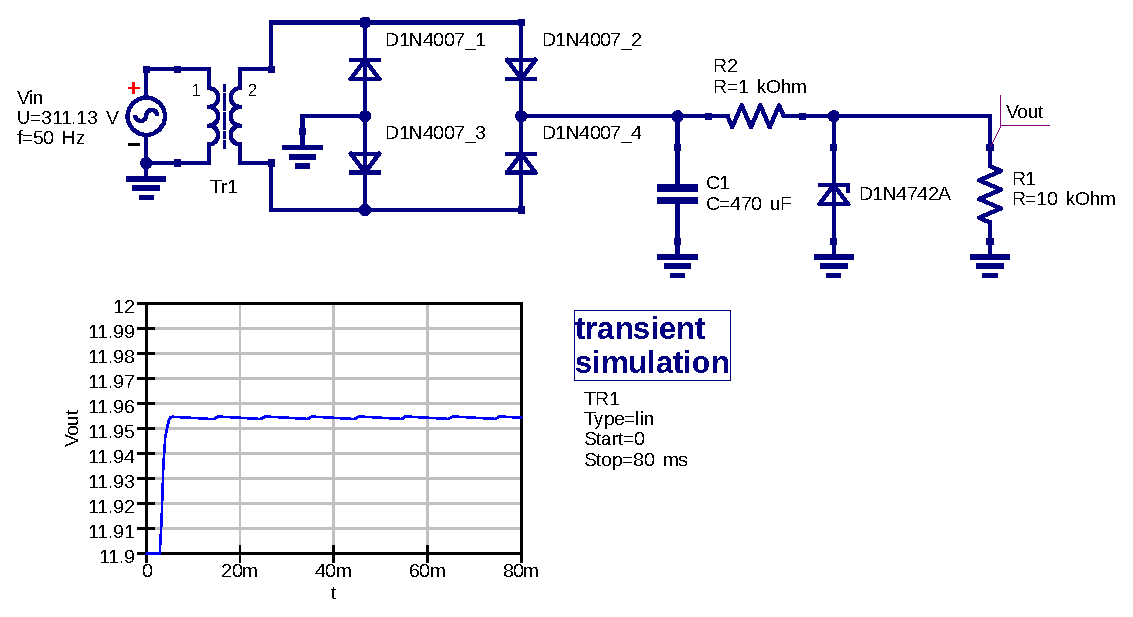
\includegraphics[scale=0.75]{simulacion/08.zener1.eps}
\caption{Simulación con el diodo \emph{Zener} \textbf{1N4742A}.}
\label{simulacion08}
\end{figure}

\subsubsection{Laboratorio}
Se presenta el regulador con diodo \emph{Zener} \textbf{1N4742A} armado en
laboratorio, su señal de voltaje de salida en osciloscopio, así como el voltaje
de la carga y las corrientes en la resistencia limitadora de
$1[\text{k}\Omega]$, diodo \emph{Zener} y resistencia de carga de
$10[\text{k}\Omega]$ en la \textbf{figura~\ref{laboratorio10}}.

\begin{figure}[!h]
\centering
\includegraphics[scale=0.26]{fotos/08.zener1.eps}
\caption{Regulador con diodo \emph{Zener} \textbf{1N4742A}.}
\label{laboratorio10}
\end{figure}


\subsection{Regulador L78XX}
La mayoría de los reguladores son circuitos integrados y tienen tres terminales:
una de entrada, una de salida y una de referencia (o ajuste). Primero se filtra
la entrada al regulador con un capacitor para reducir el rizo a $<10\%$.
Típicamente, los reguladores de voltaje proporcionan una salida constante con un
alto rechazo a los rizos.

Los reguladores de tres terminales diseñados para voltajes de salida fijos
requieren sólo capacitores externos para completar la parte de regulación de la
fuente de alimentación. El filtrado se realiza por un capacitor de gran valor
entre el voltaje de entrada y tierra. Un capacitor de salida está conectado de
la salida a tierra para mejorar la respuesta transitoria \cite{Floyd}.

En la \textbf{figura~\ref{circuito09}} se muestra un circuito regulador
\textbf{L7809CV} que fija el voltaje a $+9[\text{V}]$ filtrado por un capacitor
de $470[\mu\text{F}]$ en la entrada y un capacitor de $10[\mu\text{F}]$ para la
salida.

\begin{figure}[!h]
\centering
\includegraphics[scale=1.1]{diagramas/09.regulador1.eps}
\caption{Regulación de voltaje con \textbf{L7809CV}.}
\label{circuito09}
\end{figure}

\subsubsection{Simulación}
Se utilizó el software \emph{Quite Universal Circuit Simulator.} versión 23.3.1
para la simulación de la regulación de voltaje con el circuito integrado
\textbf{L7809CV} este puede verse en la \textbf{figura~\ref{simulacion09}}.

\begin{figure}[!h]
\centering
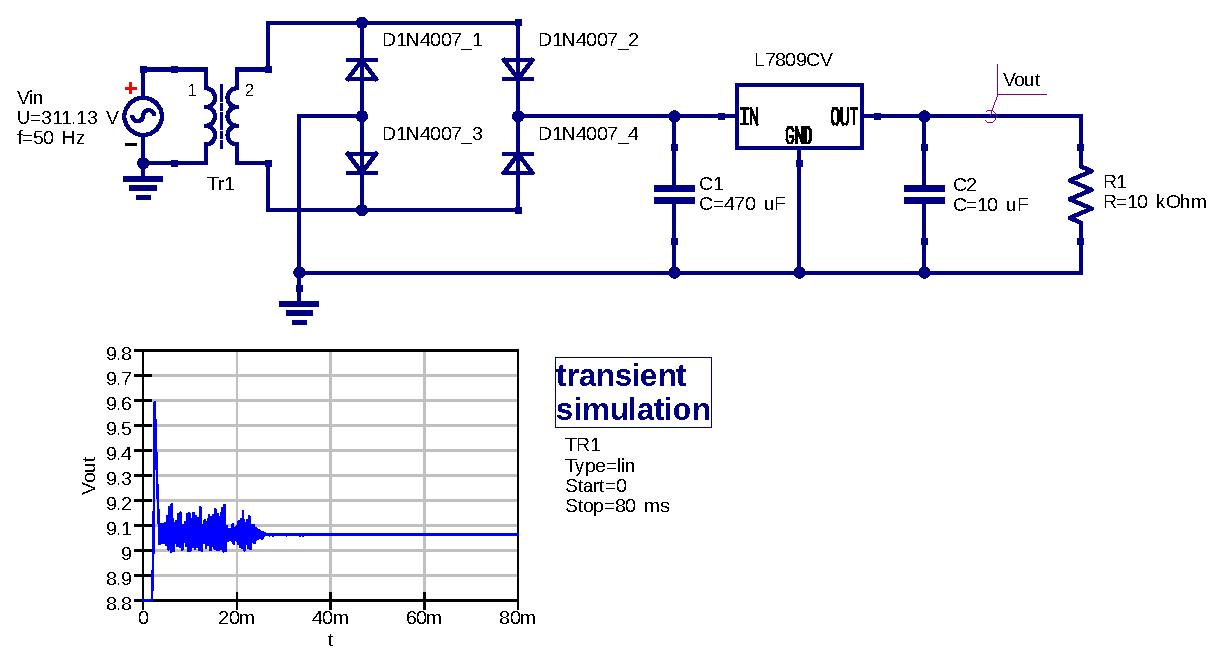
\includegraphics[scale=0.75]{simulacion/09.regulador1.eps}
\caption{Simulación del regulador \textbf{L7809CV}.}
\label{simulacion09}
\end{figure}

\begin{figure}[!h]
\centering
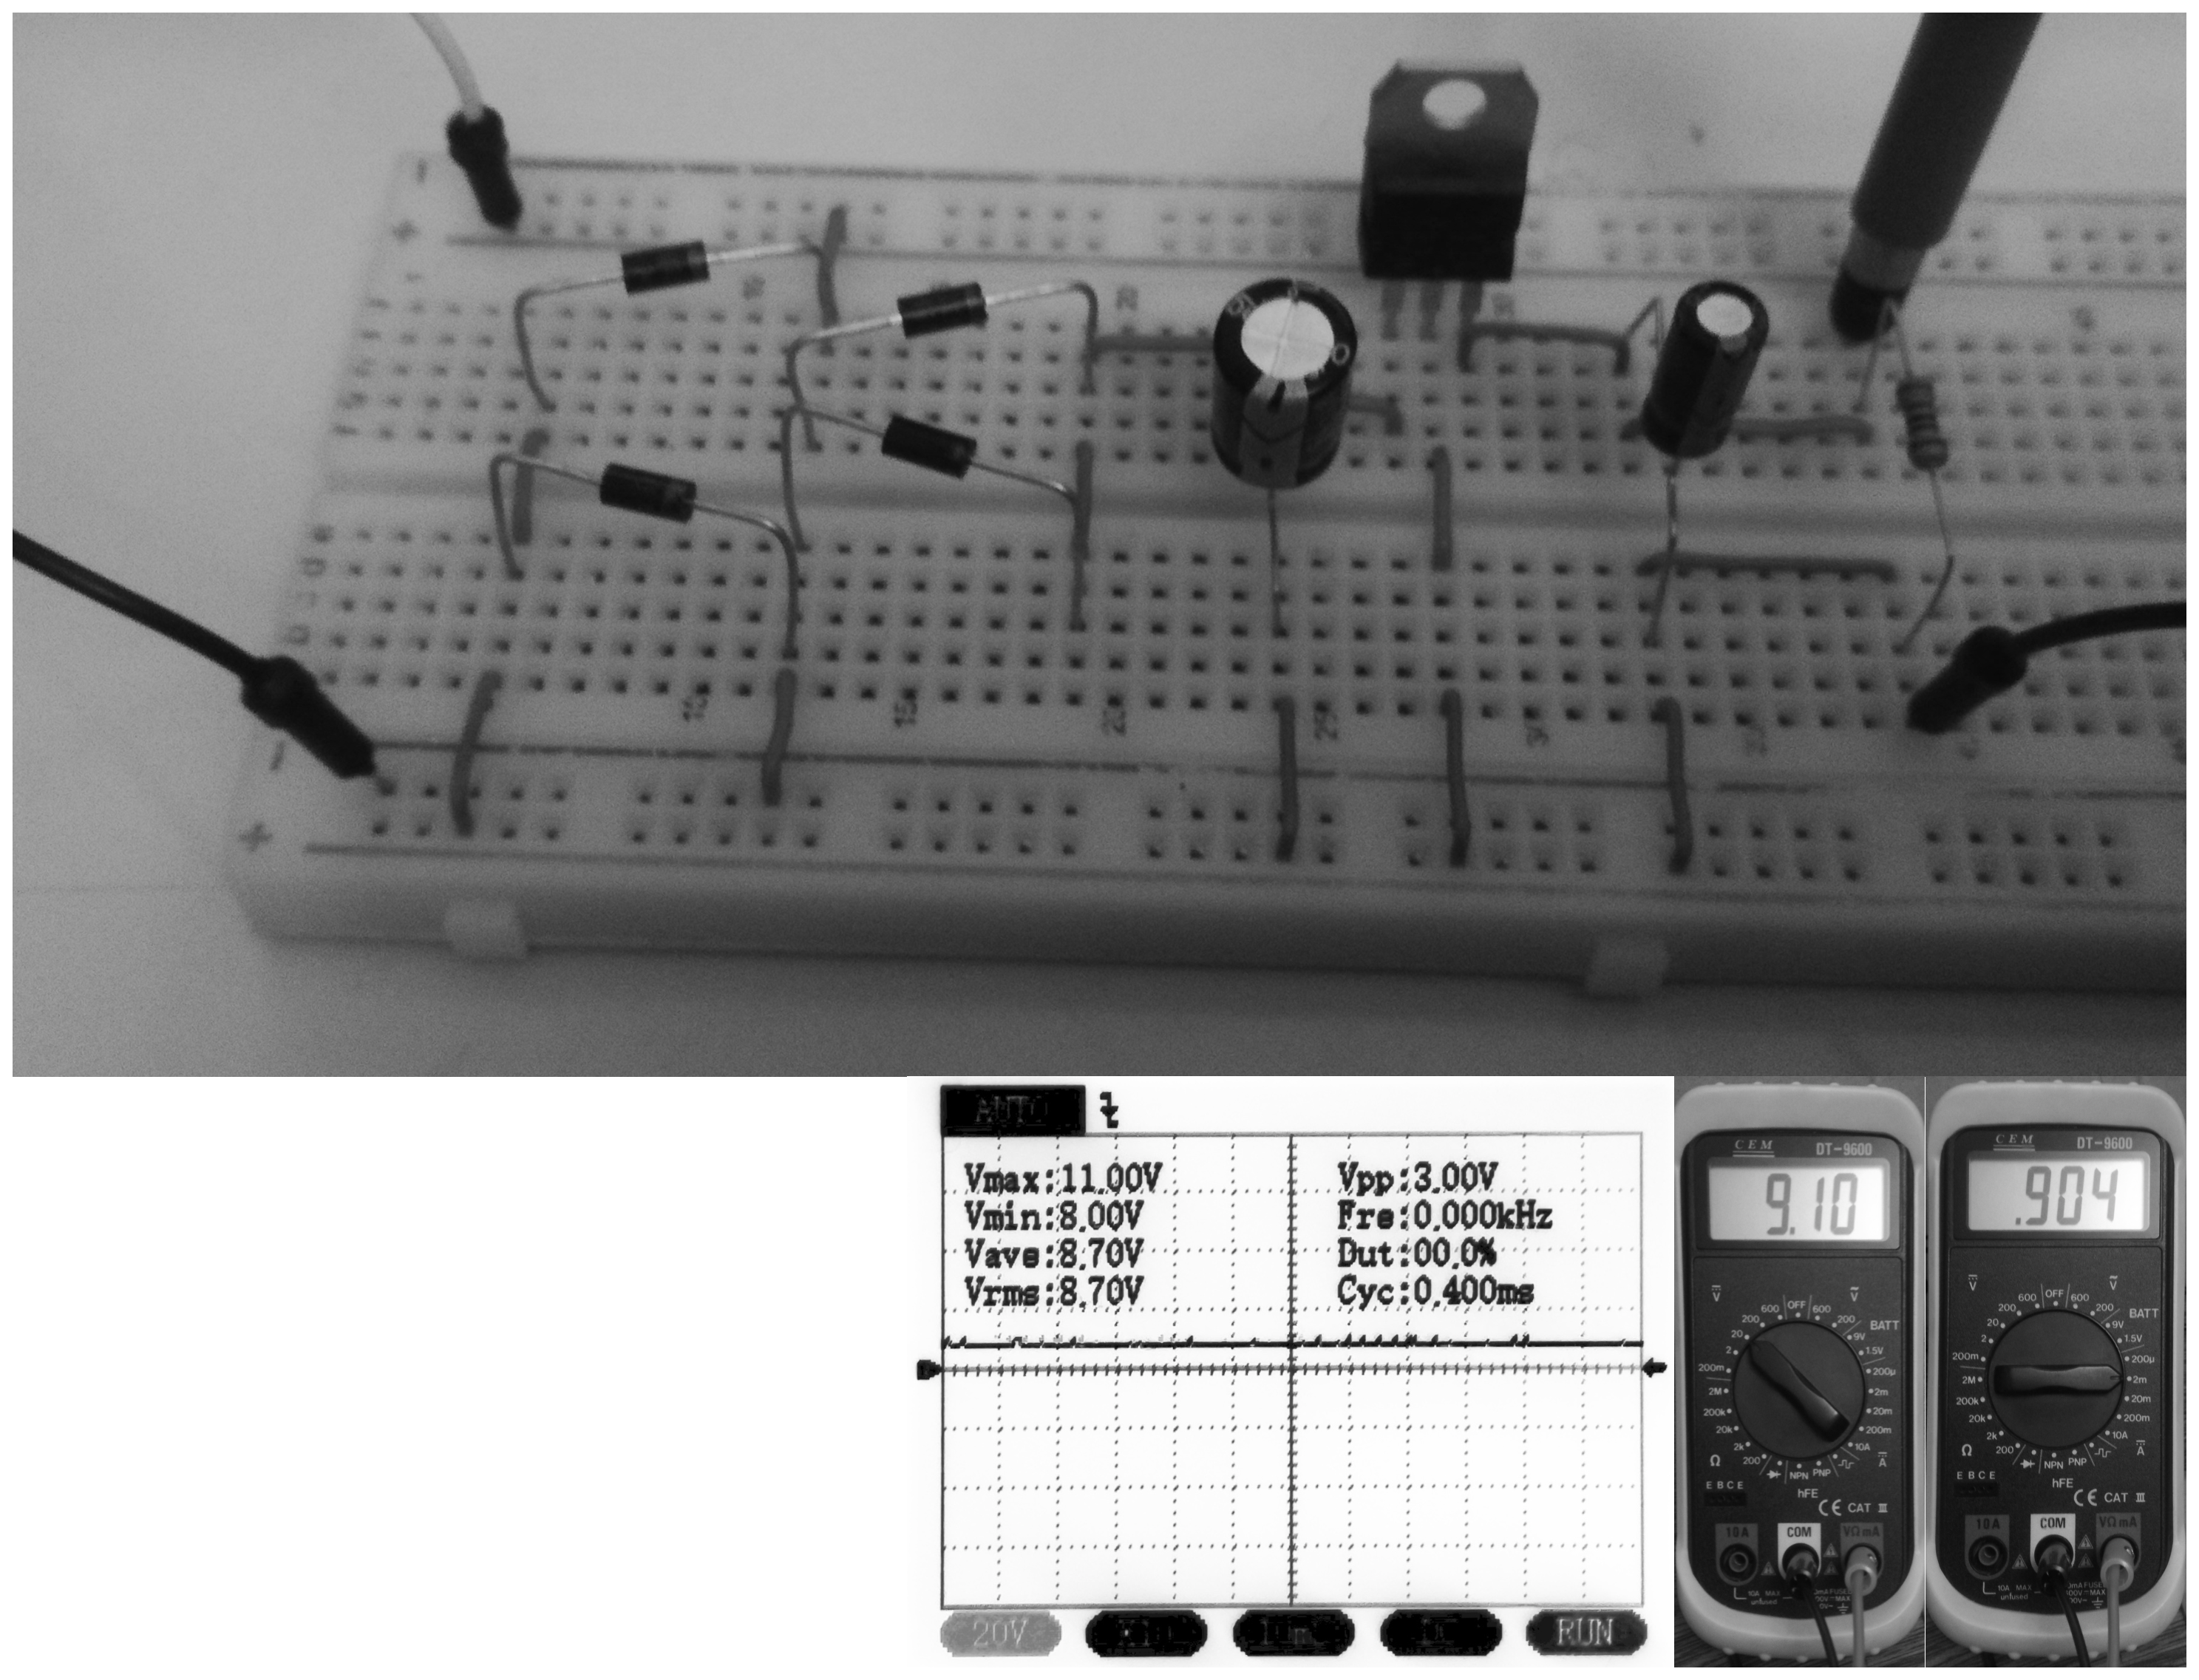
\includegraphics[scale=0.26]{fotos/09.regulador1.eps}
\caption{Regulador \textbf{L7809CV}, salida del osciloscopio\\
y medición de voltaje y corriente.}
\label{laboratorio11}
\end{figure}

\subsubsection{Laboratorio}
Se presenta el regulador \textbf{L7809CV} armado en laboratorio, su señal de
voltaje de salida en osciloscopio, así como su voltaje y corriente en un
multímetro para una resistencia de carga de $10[\text{k}\Omega]$ en la
\textbf{figura~\ref{laboratorio11}}.


\subsection{Regulador L79XX}
Además de los reguladores anteriormente mencionados, también existen reguladores
de tipo negativo que proveen una salida de voltaje inverso.

En la \textbf{figura~\ref{circuito10}} se muestra un circuito regulador
\textbf{L7909CV} que fija el voltaje a $-9[\text{V}]$ filtrado por un capacitor
de $470[\mu\text{F}]$ en la entrada y un capacitor de $10[\mu\text{F}]$ para la
salida.

\begin{figure}[!h]
\centering
\includegraphics[scale=1.1]{diagramas/10.regulador2.eps}
\caption{Regulación de voltaje con \textbf{L7909CV}.}
\label{circuito10}
\end{figure}

\subsubsection{Simulación}
Se utilizó el software \emph{Quite Universal Circuit Simulator.} versión 23.3.1
para la simulación de la regulación de voltaje con el circuito integrado
\textbf{L7909CV} este puede verse en la \textbf{figura~\ref{simulacion10}}.

\begin{figure}[!h]
\centering
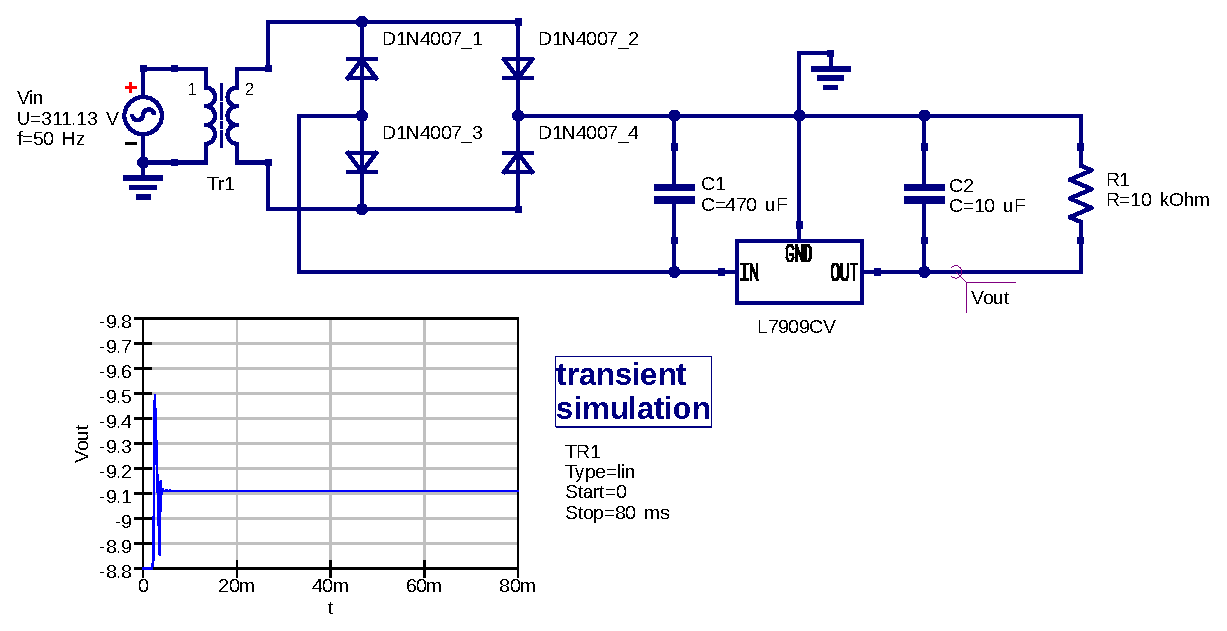
\includegraphics[scale=0.75]{simulacion/10.regulador2.eps}
\caption{Simulación del regulador \textbf{L7909CV}.}
\label{simulacion10}
\end{figure}

\begin{figure}[!h]
\centering
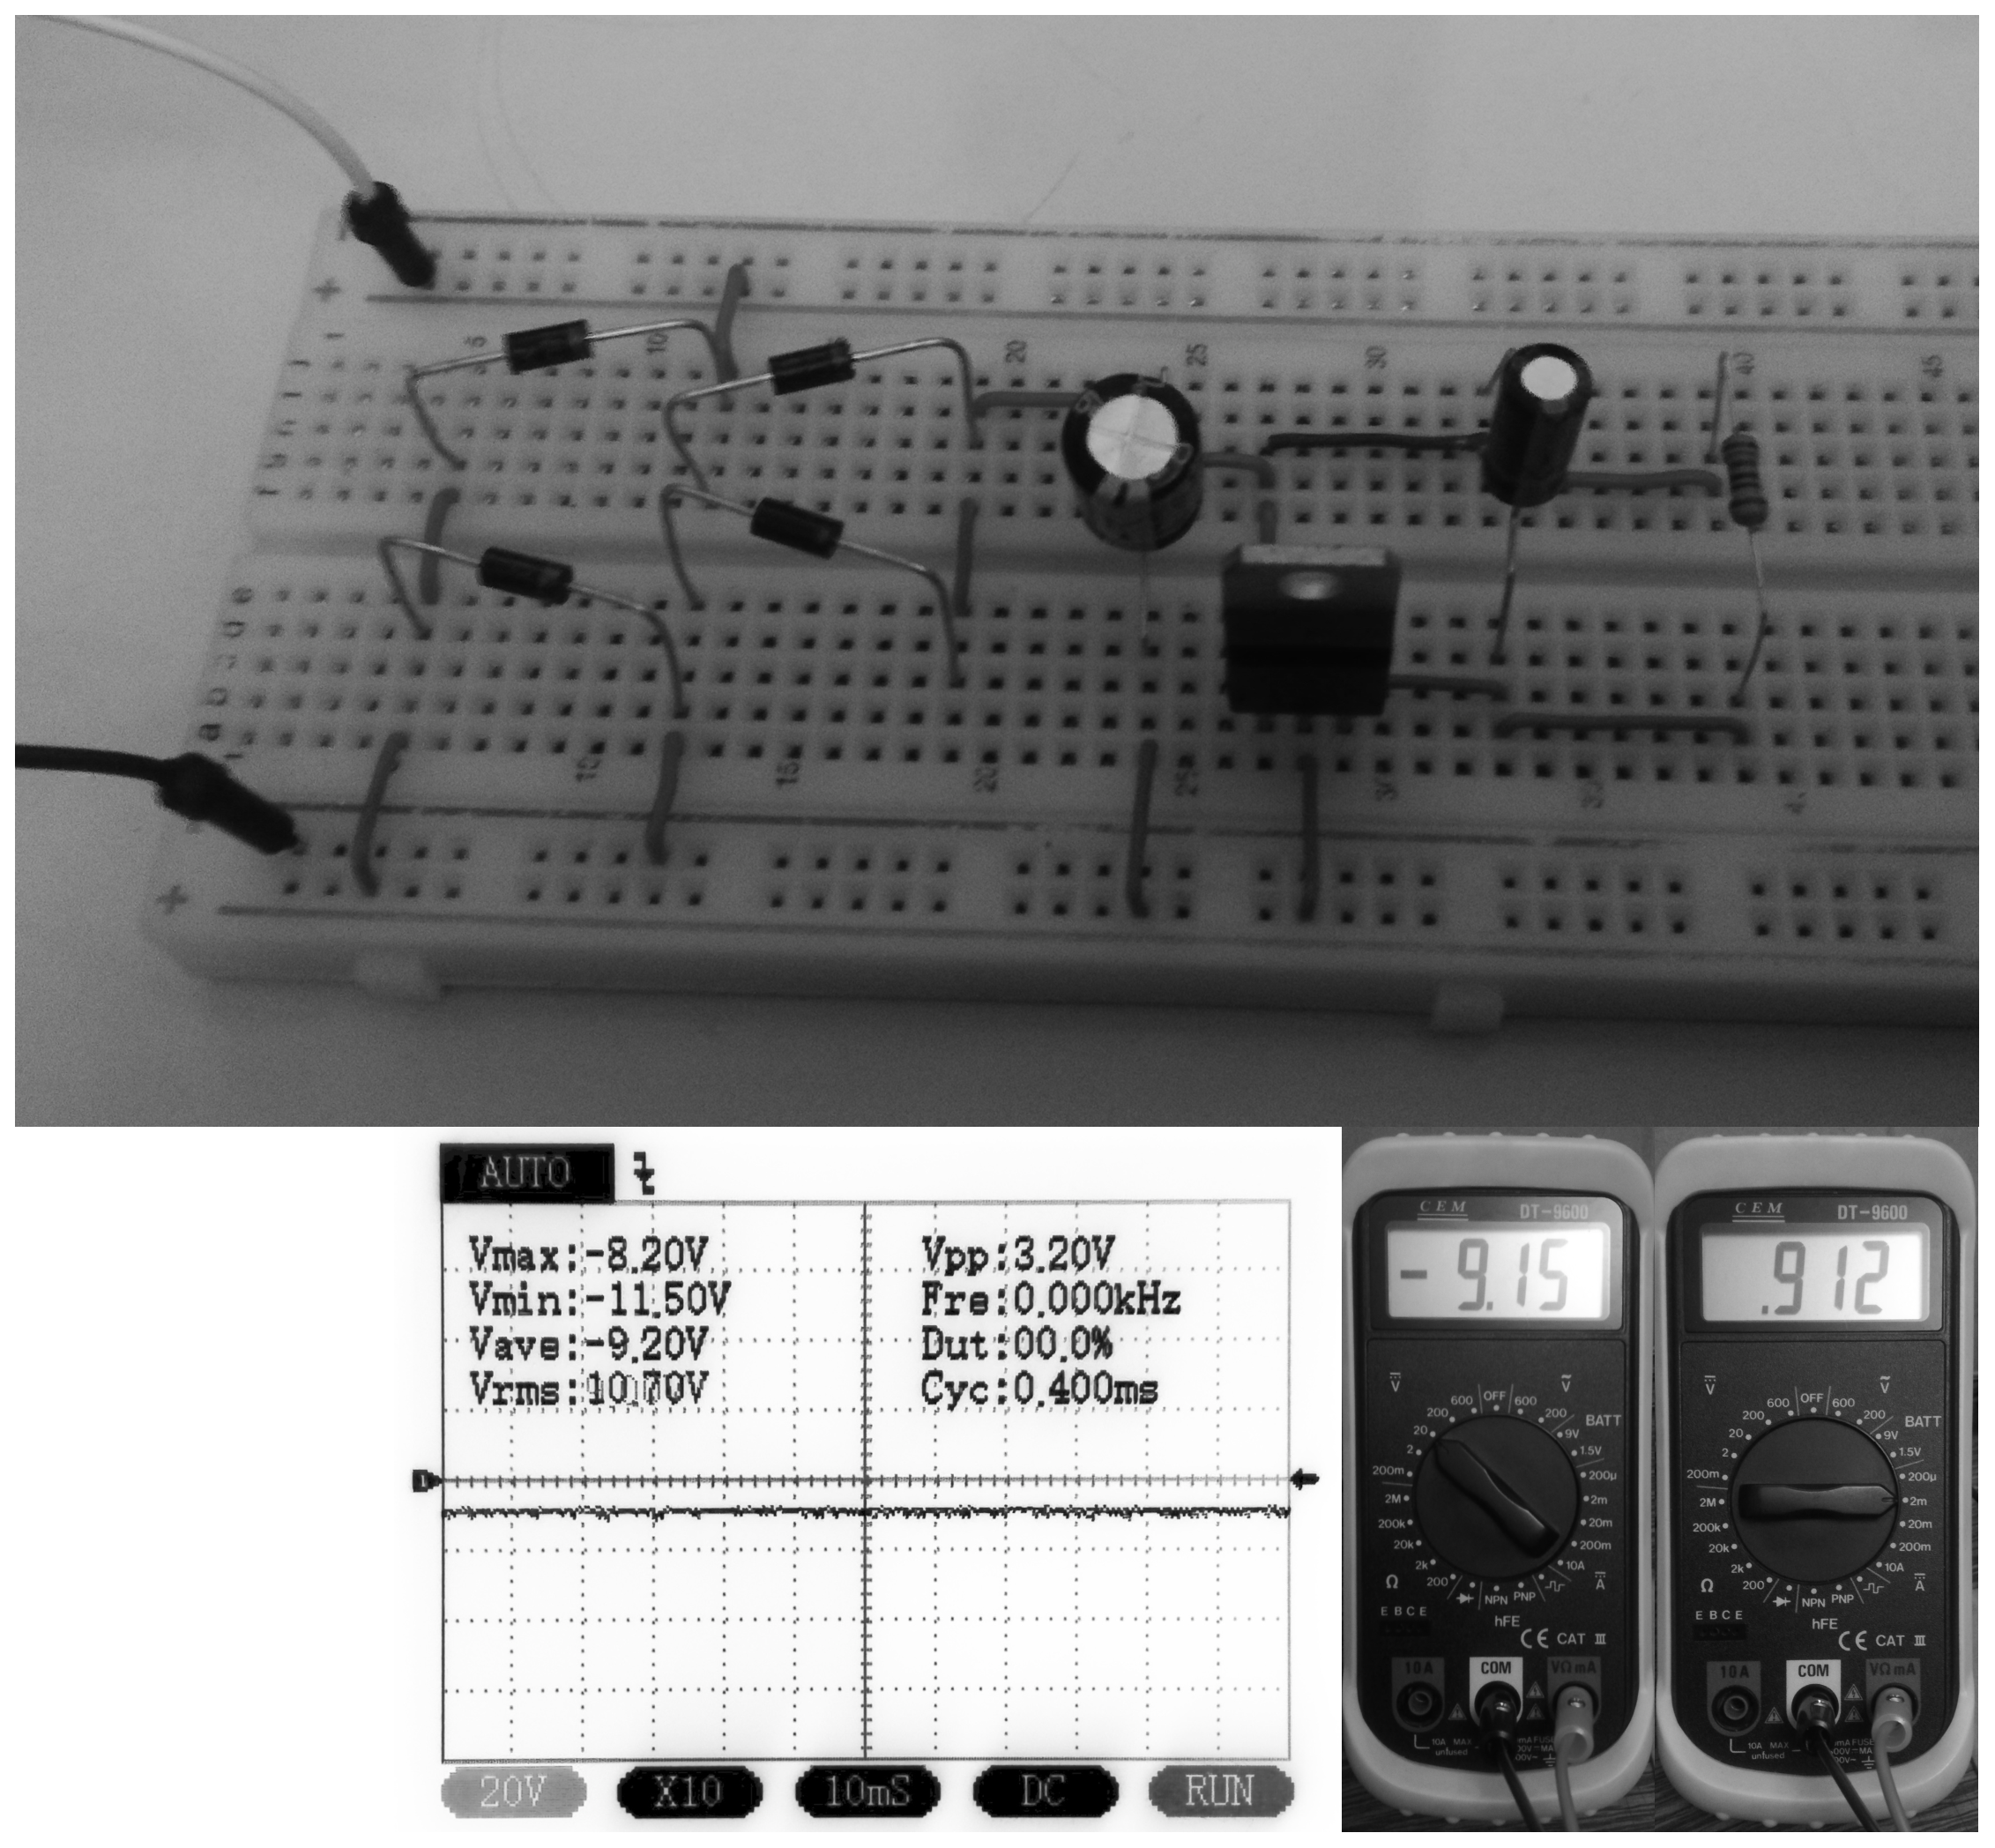
\includegraphics[scale=0.26]{fotos/10.regulador2.eps}
\caption{Regulador \textbf{L7909CV}, salida del osciloscopio\\
y medición de voltaje y corriente.}
\label{laboratorio12}
\end{figure}

\subsubsection{Laboratorio}
Se presenta el regulador \textbf{L7909CV} armado en laboratorio, su señal de
voltaje de salida en osciloscopio, así como su voltaje y corriente en un
multímetro para una resistencia de carga de $10[\text{k}\Omega]$ en la
\textbf{figura~\ref{laboratorio12}}.


\subsection{Combinación de reguladores L78XX y L79XX}
Es posible combinar ambos reguladores positivo y negativo para incrementar la
salida de voltaje, como se muestra en la \textbf{figura~\ref{circuito11}}.

\begin{figure}[!h]
\centering
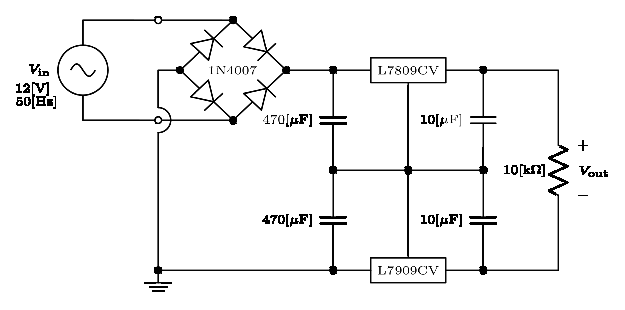
\includegraphics[scale=1.1]{diagramas/11.regulador3.eps}
\caption{Regulación de voltaje con dos circuitos integrados.}
\label{circuito11}
\end{figure}

\subsubsection{Simulación}
Se utilizó el software \emph{Quite Universal Circuit Simulator.} versión 23.3.1
para la simulación de la regulación de voltaje por medio de dos rectificadores,
este puede verse en la \textbf{figura~\ref{simulacion11}}.

\begin{figure}[!h]
\centering
\includegraphics[scale=0.75]{simulacion/11.regulador3.eps}
\caption{Simulación del regulador combinado.}
\label{simulacion11}
\end{figure}

\begin{figure}[!h]
\centering
\includegraphics[scale=0.26]{fotos/11.regulador3.eps}
\caption{Regulador combinado, salida del osciloscopio\\
y medición de voltaje y corriente.}
\label{laboratorio13}
\end{figure}

\subsubsection{Laboratorio}
Se presenta el regulador con dos circuitos integrados armado en laboratorio, su
señal de voltaje de salida en osciloscopio, así como su voltaje y corriente en
un multímetro para una resistencia de carga de $10[\text{k}\Omega]$ en la
\textbf{figura~\ref{laboratorio13}}.


\subsection{Regulación variable con L78XX}
En un regulador con circuito integrado puede hacerse una variación en el pin de
tierra para variar el voltaje de salida, conectando dos resistencias
auxiliares.

En la \textbf{figura~\ref{circuito11}} se muestra el circuito regulador de
voltaje variable con un circuito integrado \textbf{L7809CV} que fija el voltaje
a $9[\text{V}]$ y con la ayuda de un potenciómetro de $1[\text{k}\Omega]$.

\begin{figure}[!h]
\centering
\includegraphics[scale=1.1]{diagramas/12.regulador4.eps}
\caption{Regulación de voltaje variable con \textbf{L7809CV}.}
\label{circuito11}
\end{figure}

Según la ley de mallas de \emph{Kirchhoff} a la salida del regulador se tiene:
\begin{equation*}
    \begin{split}
        V_{\text{out}} &= V_{\text{reg}} + I_2\,R_2\\
    \end{split}
\end{equation*}

Según la ley de nodos de \emph{Kirchhoff} a la salida del regulador se tiene:
\begin{equation*}
    \begin{split}
        I_2 &= \left(\frac{V_{\text{reg}}}{R_1} + I_Q\right)\\
    \end{split}
\end{equation*}

Por tanto:
\begin{equation*}
    \begin{split}
        V_{\text{out}} &= V_{\text{reg}} + R_2
        \left(\frac{V_{\text{reg}}}{R_1} + I_Q\right)\\
    \end{split}
\end{equation*}

La variación del voltaje de salida varia desde $9[\text{V}]$ para un valor de
$0[\Omega]$ en la resistencia variable, hasta el máximo que provee el
rectificador para el valor de $1[\text{k}\Omega]$.

\subsubsection{Simulación}
Se utilizó el software \emph{Quite Universal Circuit Simulator.} versión 23.3.1
para la simulación de la regulación de voltaje variable con el circuito
integrado \textbf{L7809CV}, un potenciómetro de $1[\text{k}\Omega]$, una
resistencia fija $R_1 = 9[\text{k}\Omega]$ y una resistencia de carga de
$R_{\text{out}} = 10[\text{k}\Omega]$. este puede verse en la
\textbf{figura~\ref{simulacion12}}.

\begin{figure}[!h]
\centering
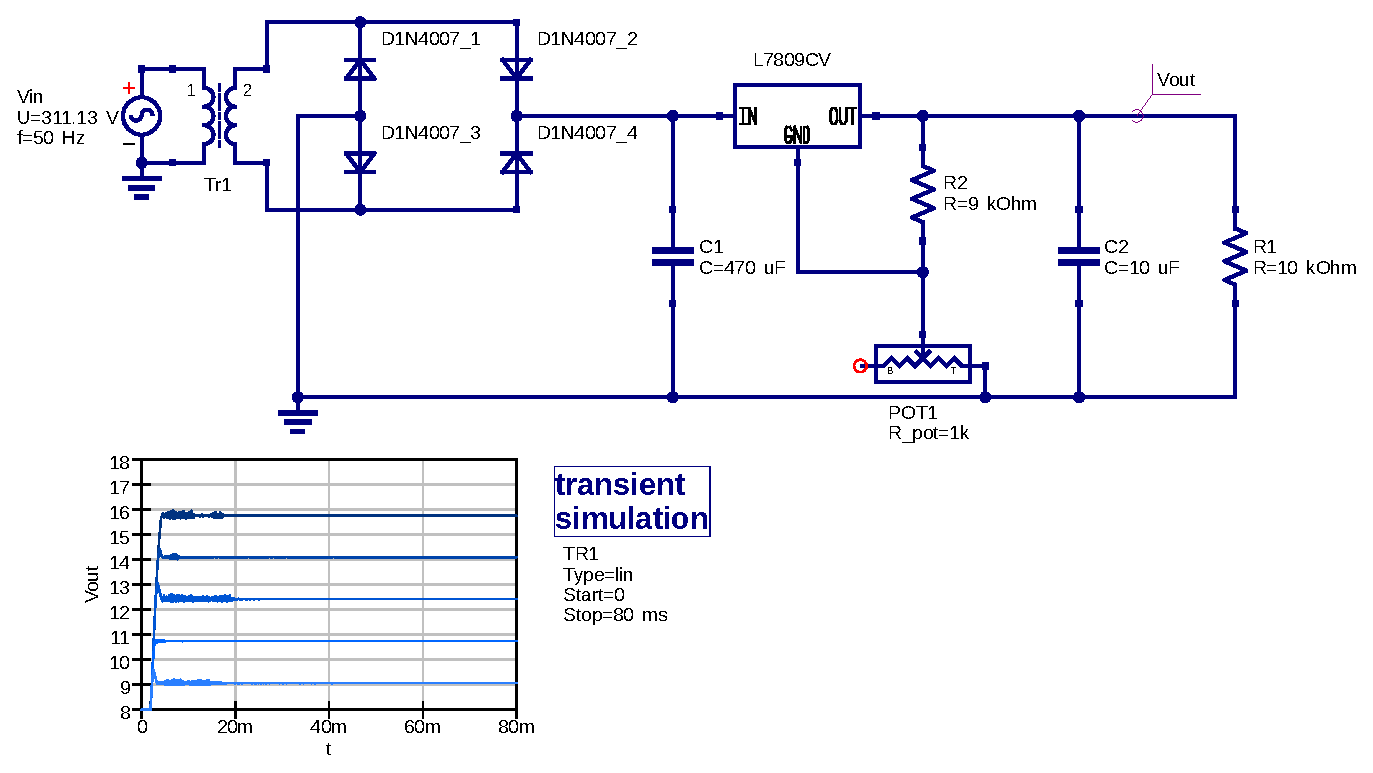
\includegraphics[scale=0.75]{simulacion/12.regulador4.eps}
\caption{Simulación del regulador variable con \textbf{L7809CV}.}
\label{simulacion12}
\end{figure}

\begin{figure}[!h]
\centering
\includegraphics[scale=0.28]{fotos/12.regulador4.eps}
\caption{Regulación variable con \textbf{L7809CV} \\
y medición de corriente y voltaje.}
\label{laboratorio14}
\end{figure}

\subsubsection{Laboratorio}
Se presenta el regulador \textbf{L7809CV} armado en laboratorio, así como su
voltaje y corriente en un multímetro para los valores de resistencia variable de
$0[\Omega]$ y $1[\text{k}\Omega]$, este puede verse en la
\textbf{figura~\ref{laboratorio14}}.


\section{Conclusiones y Recomendaciones}
Se comprobó el funcionamiento de los transformadores con derivación central, y
lo importante del uso de un fusible en los experimentos.

Se verificaron los comportamientos de los rectificadores tanto de media onda, de
onda completa con un transformador con derivación central y de onda completa con
puente.

Se verificaron los comportamientos de los filtros a la salida del rectificador y
como estos son importantes para la eliminación de rizos.

Se comprobaron los diferentes tipos de regulación de voltaje que pueden ser
utilizados para una fuente de alimentación de corriente directa.

A su vez, de los componentes electrónicos de los diferentes circuitos armados
es crucial hacer una revisión de sus hojas de datos, para evitar que el diseño
exceda sus valores recomendados de funcionamiento.



\begin{thebibliography}{99}

\bibitem{Floyd}
Thomas L. Floyd (208).\\
\textbf{Dispositivos electrónicos. 8va Edición.}\\
Pearson Education\\

\bibitem{Fiore}
James M. Fiore (2017).\\
\textbf{Dispositivos semiconductores. Teoría y aplicación.}\\
Mohawk Valley Community College\\
Extraído el 12 de Octubre del 2024, de: \\
\url{https://espanol.libretexts.org/Ingenieria/Libro%3A_Dispositivos_semiconductores_-_Teor%C3%ADa_y_Aplicaci%C3%B3n_(Fiore)/03%3A_Aplicaciones_de_diodos/3.2%3A_Rectificaci%C3%B3n}

\end{thebibliography}

\end{document}

